\section{Interactive Dashboard}
\label{sec:dashboard}

The dashboard exposes the queries in Section~\ref{sec:sql} to a non-SQL
audience. It is a Streamlit \cite{streamlit} application that connects
directly to the PostgreSQL database described in Section~\ref{sec:dbsetup}
and renders results with Plotly \cite{plotly}. All charts are
parameterized by sidebar filters; selecting a host or attack phase
re-issues the underlying SQL and updates every chart on the page.

\subsection{Architecture}
The application is a single-page Streamlit app structured as:

\begin{verbatim}
src/dashboard/
|-- app.py        Streamlit entry point, layout, charts
|-- db.py         psycopg2 connection helper
`-- queries.py    parameterized SQL strings
\end{verbatim}

The runtime path on every page render is: user input on the sidebar
$\rightarrow$ Streamlit re-runs \texttt{app.py} $\rightarrow$
\texttt{queries.py} produces a parameterized \texttt{SELECT}
$\rightarrow$ \texttt{db.py} executes against PostgreSQL $\rightarrow$
result returned as a Pandas DataFrame $\rightarrow$ Plotly figure
constructed and rendered. This mirrors the Lecture-11 Flask + PyMySQL +
Chart.js pattern, with Streamlit + psycopg2 + Plotly substituted for the
equivalent layers.

\subsection{Visualizations}
Eight charts are wired to the database. Each chart is bound to a single
SQL query (or the persisted view in Section~\ref{sec:sql}) and the
caption names the source query so the linkage to the SQL portfolio is
explicit.

\begin{enumerate}
  \item Bar chart: labeled lines per host. Source: B1. % River
  \item Bar chart: labels per attack phase. Source: B4. % Ishaan
  \item Horizontal bar: top-10 detection rules. Source: B5. % Ishaan
  \item Heatmap: events per day per host with rank highlight.
    Source: A3. % Ishaan
  \item Stacked bar: \texttt{(source\_host, source\_log)} share of
    labeled lines. Source: A2. % River
  \item Service-activity table with sparklines. Source: B6. % Naman
  \item Filterable attack timeline. Source: persisted view
    \texttt{v\_attack\_timeline}. % Naman
  \item Phase-vs-source coverage heatmap. Source: B-Naman-Q2 (4-table
    join with \texttt{COUNT DISTINCT}).
\end{enumerate}

\subsection{Filters}
The sidebar exposes two filters:
\begin{itemize}
  \item \texttt{host\_key} (multi-select, default = all 22 hosts).
  \item \texttt{attack\_phase} (multi-select, default = all 7 phases).
\end{itemize}
Both filters are applied as \texttt{WHERE} clauses on the
\texttt{host} and \texttt{attack\_phase} joins. Charts that do not
depend on those joins (B2: phase taxonomy) ignore the filter value
gracefully.

\subsection{Demo}
% TODO: insert figures/dashboard_overview.png
% TODO: insert figures/dashboard_filter_demo.png
Figure \ref{fig:dashboard-overview} shows the default view. Figure
\ref{fig:dashboard-filter} shows the same dashboard after filtering to
\texttt{intranet\_server} only, which collapses charts 1, 4, 6, 7, and 8
to the privilege-escalation evidence on a single host. The dashboard
runs locally with \texttt{streamlit run src/dashboard/app.py} after the
load steps in Section~\ref{sec:dbsetup}.

\begin{figure}[htbp]
\centering
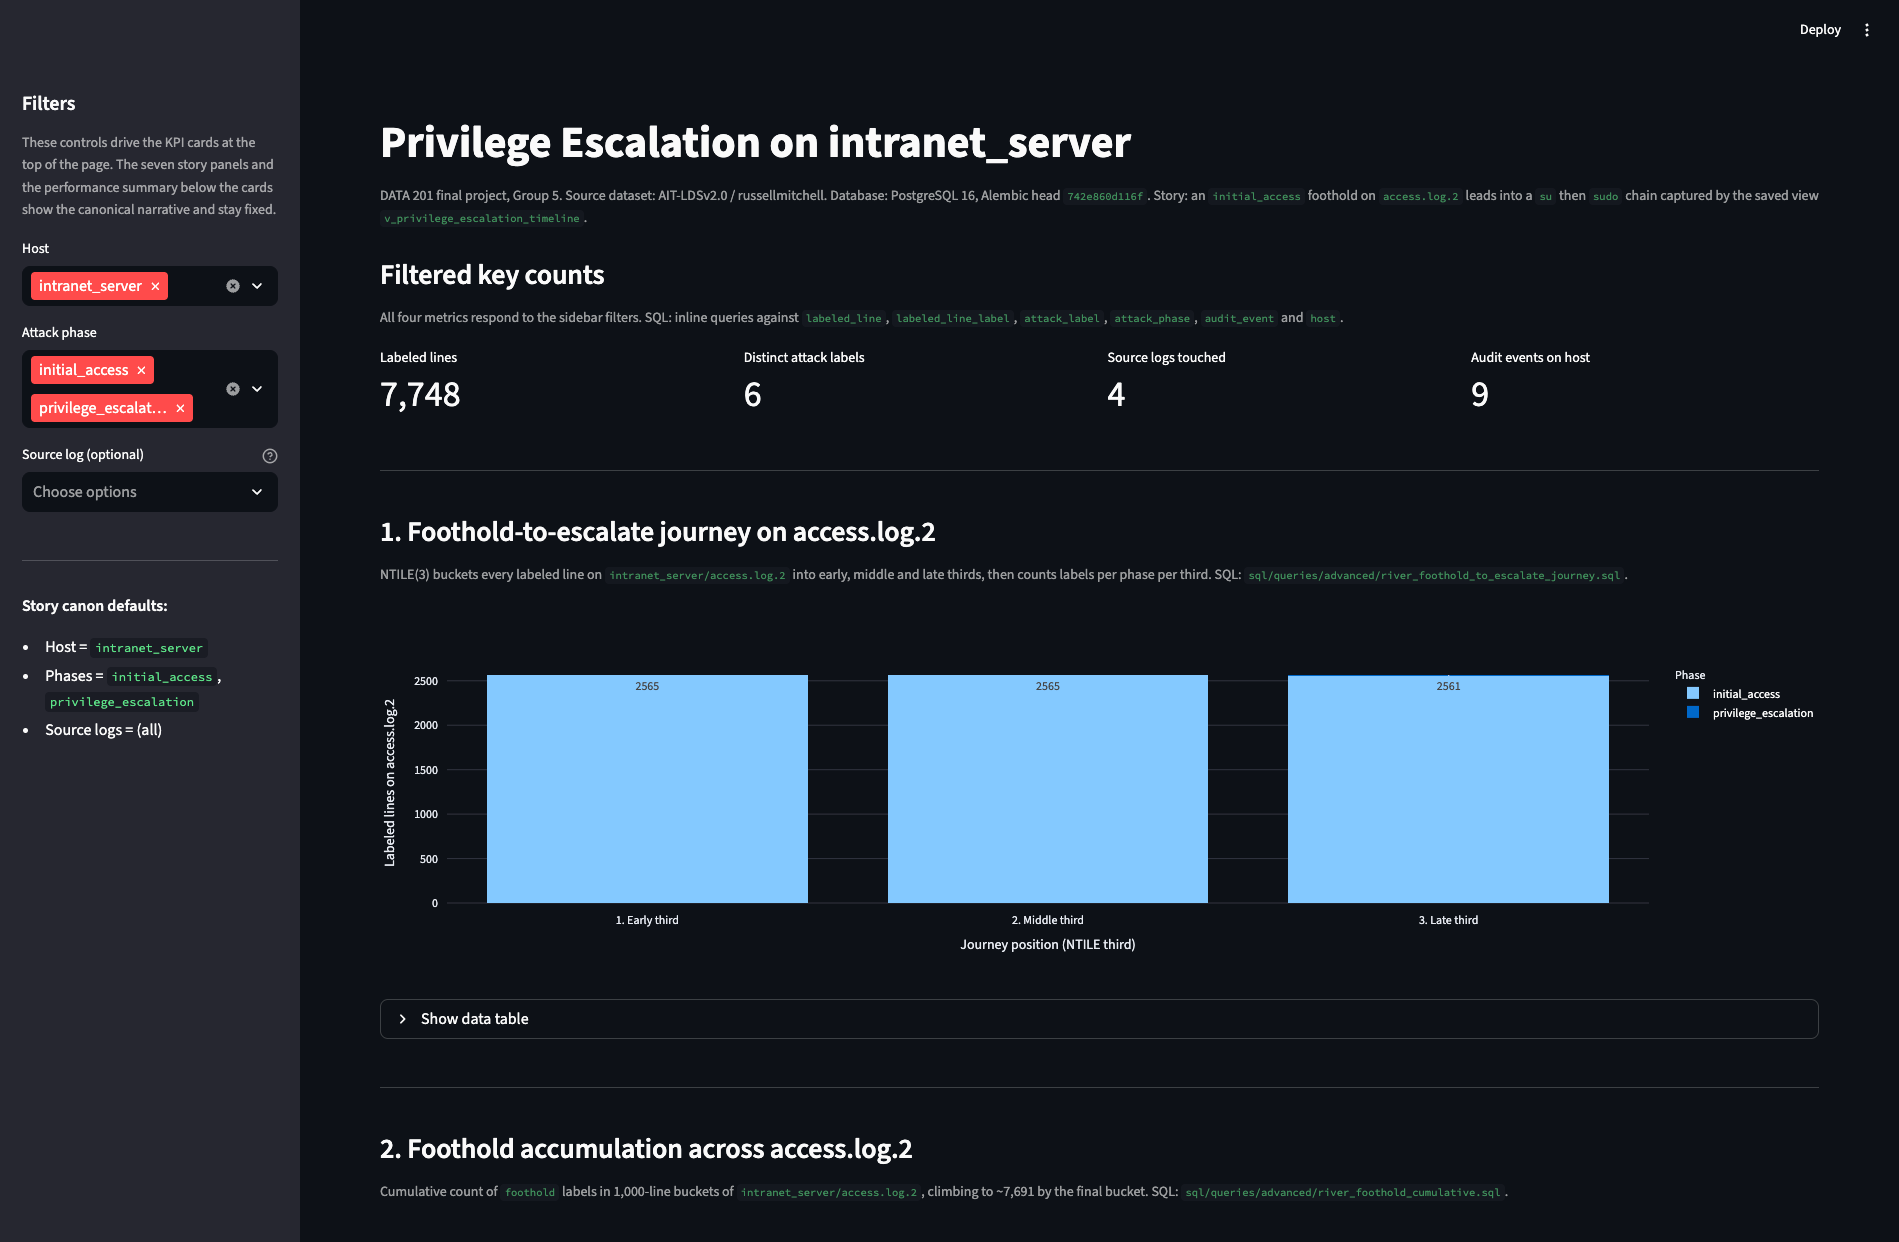
\includegraphics[width=\columnwidth]{figures/dashboard_overview.png}
\caption{Dashboard default view, no filters applied. Eight charts wired
  to the queries in Section~\ref{sec:sql}.}
\label{fig:dashboard-overview}
\end{figure}

\begin{figure}[htbp]
\centering
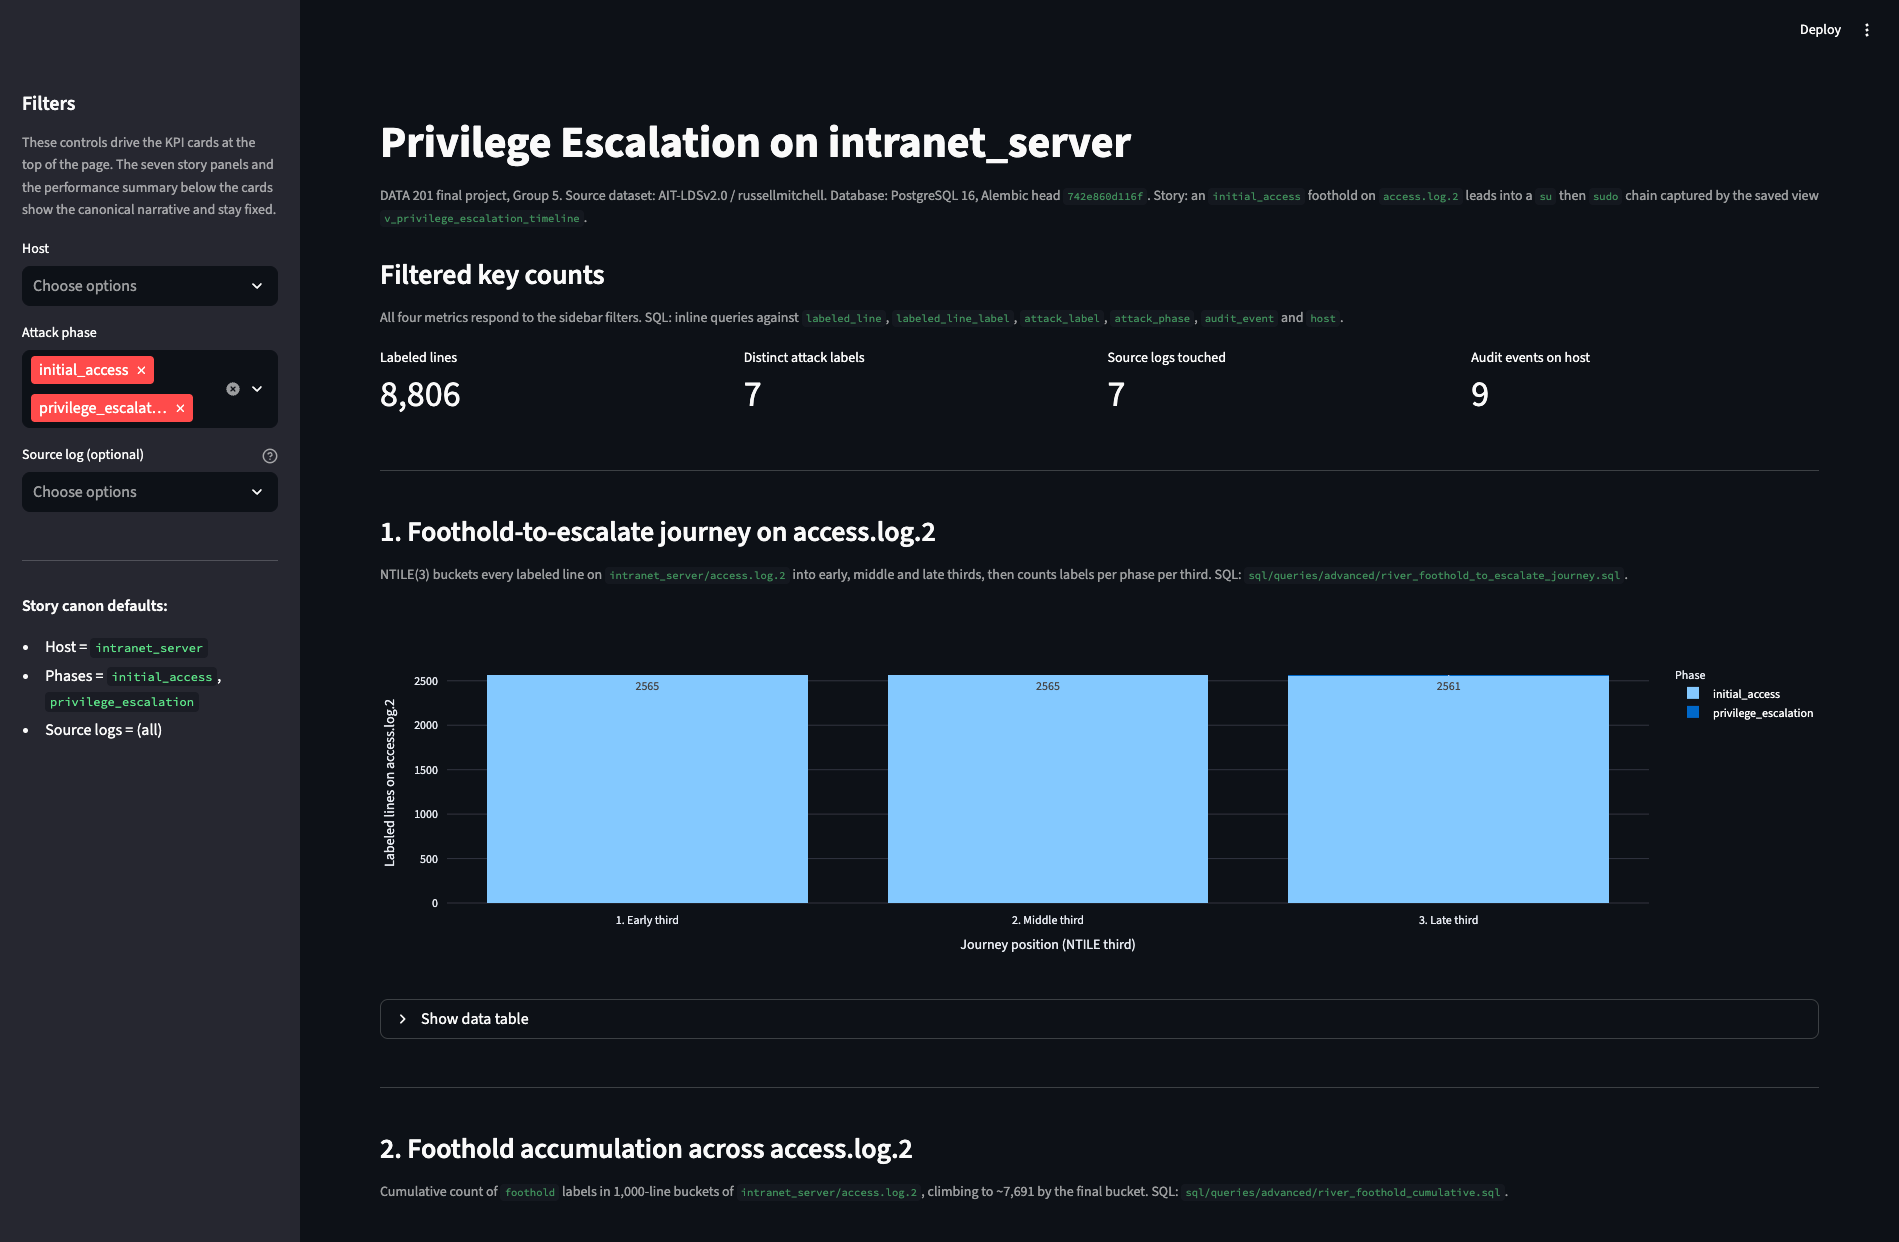
\includegraphics[width=\columnwidth]{figures/dashboard_filter_demo.png}
\caption{Dashboard after filtering to \texttt{intranet\_server}. Charts
  1, 4, 6, 7, and 8 update; charts 2, 3, and 5 (taxonomy / global
  detection-rule volume) are intentionally invariant.}
\label{fig:dashboard-filter}
\end{figure}
